%======================================================================================
\chapter{The Standard Model and the Higgs Boson}
%======================================================================================

\section{The Standard Model Structure}
The Standard Model (SM) is a set of quantum field theories, locally gauge invariants, that describes the interactions\footnote{Except the gravity which is not described by the SM currently.} between the fundamental particles building the known matter. Such interactions arise by requiring the gauge symmetry on the lagrangians of the theories contained into the SM. These theories are the Quantum Electrodynamic (QED), the Glashow-Weinberg-Salam (GWS - electroweak interaction) and the Quantum Chromodynamic (QCD). The QED is based on the symmetry group $U(1)$ and describes the electromagnetic interactions between charged particles. The GWS is the theory describing the electroweak processes, such as the particles decays, and is based on the symmetry group $SU(2)_L \times U(1)_Y$. The QCD is structured on the symmetry group $SU(3)_C$ and describes the strong interaction, which is responsible, for instance, to keep the atomic nucleon stable \cite{bib:whitbeck-2013, bib:brachem-2012}.

Based on the fact that all the known matter is constituted of elementary particles which interacts in different ways between them, the SM organizes such particles in several classes, with the most elementary ones being: quarks, leptons and bosons. The quarks do not appear alone in nature as far it is known. These particles are always observed in pairs or triplets forming particles classified as mesons (quark-antiquark pair) and barions (triplets of quarks and antiquarks). The barions and mesons are grouped into another class called hadrons. Examples of mesons are the pions and kaons produced in collision experiments and in cosmic rays and, examples of barions are the protons and neutrons \cite{bib:griffiths-2008,bib:halzen-martin-1984}.

The leptons and quarks are together classified as fermions because they have fractioned quantum number of spin and are divided into six flavors organized in doublets in the SM. Such doublets are often identified in three generations. The ordinary matter is composed by the quarks of first generation while the other ones appear in particles produced in accelerators or cosmic rays, for instance. The leptons can interact weakly and electromagnetically (except the neutrinos which only interact weakly), while the quarks can interact through any of the three SM interactions (since they have electric and color charge). The color charge is another quantum number that has been introduced originally in order to fit the existence of particles composed by three quarks of same flavor (the case of $\Omega^-$). Without this consideration the Pauli exclusion principle avoids the existence of such particle. There are three color charges for each quark and often they are referred as red, yellow and blue, in analogy to the primary colors which combined produce the white (no color), similar to the hadrons that do not have color charge \cite{bib:griffiths-2008,bib:halzen-martin-1984}.

The bosons are the interaction mediators between the elementary particles and present integer quantum numbers of spin. The mediator of the strong interaction are the non-massive gluons (g), which interacts with color charged particles and themselves, exiting in 8 types. The electromagnetic interaction is mediated by the non-massive photon ($\gamma$), which does not have electric charge and thus do not self interact. Associated to the weak interaction there are three massive bosons, two charged ($W^{\pm}$) and one neutral ($Z$). The Tab.~\ref{tab:TabParticulas} summarizes the properties of the elementary particles and their interactions described by the SM.

\begin{table}[htbp]{16cm}
\caption{Elementary particles and their interactions in the SM.}
\centering
\begin{tabular}{ccccc}
\hline \hline
Generation & Flavor 							& Charge [$e$]  & Mass [MeV] 	& Lifetime [s]\\
\hline
		   &		 							& Leptons 	    &	   		   	& \\
\hline
$1ª$    & $e$ (electron) 					& -1  			& 0.51    		& 1.4*$10^{34}$ \\
		& $\nu_e$ (neutrino do $e$) 		& 0 			& $\approx 0$ 	& - \\
$2ª$	& $\mu$ (muon)  					& -1  			& 105.66  		& 2.2*$10^{-6}$ \\
		& $\nu_{\mu}$ ($\mu$ neutrino) 	    & 0 			& $\approx 0$ 	& - \\
$3ª$	& $\tau$ (tau) 						& -1  			& 1776.82 		& 2.9*$10^{-13}$ \\
		& $\nu_{\tau}$ ($\tau$ neutrino)    & 0 			& $\approx 0$ 	& - \\
\hline
		&		        & Quarks  	 &	   		   & \\
\hline
$1ª$	& $u$ (up)      & 2/3   & 2.30  	& - \\
		& $d$ (down)    & -1/3  & 4.80  	& - \\
$2ª$	& $c$ (charm)   & 2/3	& 1275.00 	& - \\
		& $s$ (strange) & -1/3  & 95.00   	& - \\
$3ª$	& $t$ (top)		& 2/3	& 173500.00 & - \\
		& $b$ (bottom)  & -1/3  & 4180.00 	& - \\
\hline
		        &		 		   & Bosons  	&	   		 & \\
\hline
Interaction 	& Associated   & Charge [$e$] & Mass [GeV] & Coupling\\
				& Boson		   &			&			   & Strength\\
\hline
Nuclear Strong  & $g$ (8 gluons)   & 0       	& 0     	 & 1\\
Nuclear Weak    & $W^{\pm}$		   & $\pm$ 1 	& 80.38 	 & $10^{-6}$\\
				& $Z$  		   	   & 0		 	& 91.19 	 &\\
Electromagnetic & $\gamma$ (photon) & 0 		 	& 0     	 & $10^{-2}$\\
\hline \hline
\end{tabular}
\source{GRIFFITHS, 2008, p. 12; HALZEN, 1984, p. 26; BERINGER, 2012, p. 27-33. Adapted by the author.}
\label{tab:TabParticulas}
\end{table}

Although the SM has shown great success in the description of the elementary particles and their interactions, the method of introducing such interaction by requiring the gauge symmetries created a divergence with the observations. The gauge symmetry does not allow mass terms in the SM theory. However, since Glashow, proposing the $SU(2)$ structure for the electroweak interactions, it was known that the boson $W$ has mass. This inconsistency was solved by the so called Higgs mechanism, which states the existence of a scalar boson (spin 0) whose interaction with the elementary particles generates their mass through the process known as Spontaneous Symmetry Breaking (SSB) \cite{bib:whitbeck-2013,bib:griffiths-2008}.

\section{Spontaneous Symmetry Breaking}
The spontaneous symmetry breaking is a phenomenon not restricted to the Particle Physics. In such context, though, it can be used as a mechanism to introduce mass terms in the SM theory without violating the gauge symmetries. It is important to highlight that different aspects can be observed for different situations when applying the SSB. As a general illustration, consider the following lagrangian for two scalar fields $\phi_1$ and $\phi_2$ (Goldstone Model) given by

\begin{equation}
\mathcal{L} = \dfrac{1}{2}[(\partial_{\mu}\phi_1)^2 + (\partial_{\mu}\phi_2)^2 ] - V(\phi_1^2 + \phi_2^2)
\label{eq:Goldstone_potential}
\end{equation}  

which is invariant under transformations of the SO(2) rotation group

\begin{equation}
\phi \equiv \left(\begin{aligned} \phi_1 \\ \phi_2 \end{aligned} \right) \rightarrow \left(\begin{aligned} cos \!\ \theta \quad sen \!\ \theta \\ -sen \!\ \theta \quad cos \!\ \theta \end{aligned} \right) \left(\begin{aligned} \phi_1 \\ \phi_2 \end{aligned} \right). 
\end{equation}

Now, suppose a potential for the lagrangian in the following form

\begin{equation}
V(\phi^2) = \dfrac{1}{2}\mu^2 \phi^2 + \dfrac{1}{4} \vert \lambda \vert (\phi^2)^2
\end{equation}

where, $\phi^2 = \phi_1^2 + \phi_2^2$. The choice of the parameter $\mu$ defines two distinguishable cases for the potential. The case $\mu^2 > 0$ corresponds to the exact symmetry, with the vacuum state occurring for

\begin{equation}
\langle \phi \rangle = \left(\begin{aligned} 0 \\ 0 \end{aligned} \right)
\end{equation}

and the potential in this case has the profile represented in Fig.~\ref{fig:muPotencial}(a). The lagrangian, in such condition, describes just a pair of scalar particles with common mass $\mu$. The case $\mu^2 < 0$ leads to the spontaneous breaking of the symmetry SO(2), in which the absolute minimum of the potential, Fig.~\ref{fig:muPotencial}(b), corresponds to different vacuum states (all degenerated in energy) given by

\begin{equation}
\langle \phi_0 \rangle = - \dfrac{\mu^2}{\vert \lambda \vert} = v^2
\end{equation}

\begin{figure}[htbp]{15cm}
\caption{The $V(\phi)$ potential for different choices of $\mu^2$.}
\subfloat[]{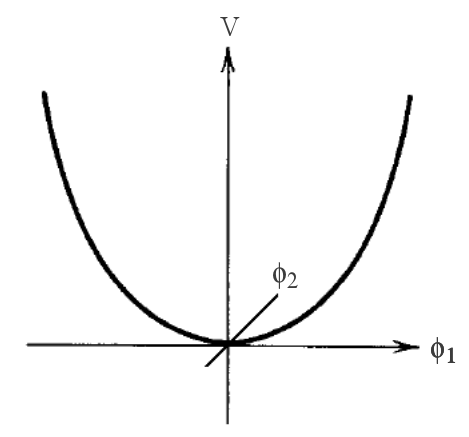
\includegraphics[scale=0.4]{ChapterTheory/figs/mu_pos.png}} \quad \quad
\subfloat[]{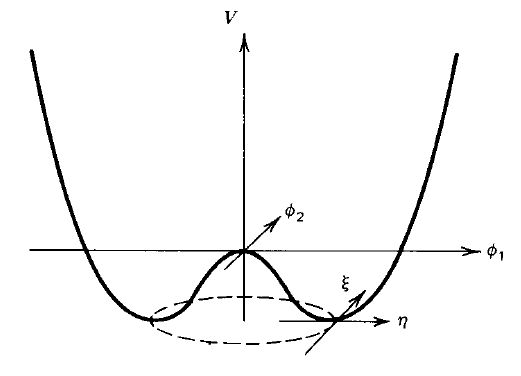
\includegraphics[scale=0.34]{ChapterTheory/figs/mu_neg.png}}
\legend{(a) $\mu^2 > 0$; (b) $\mu^2 < 0$.}
\source{HALZEN, 1984, p. 322 and 325. Adapted by the author.}
\label{fig:muPotencial}
\end{figure}

Considering now one of those vacuum states (in terms of $\phi_1$ and $\phi_2$) and making the expansion around the chosen state, one has

\begin{eqnarray}
\langle \phi \rangle &=& \left(\begin{aligned} v \\ 0 \end{aligned} \right) \\ \phi' &\equiv& \phi - \langle \phi_0 \rangle \quad \rightarrow \quad \langle \phi \rangle = \left(\begin{aligned} v +& \eta \\ \xi& \end{aligned} \right).
\end{eqnarray}

Inserting this new displaced field in the lagrangian, it becomes

\begin{equation}
\mathcal{L} = \dfrac{1}{2}[(\partial_{\mu}\eta)^2 + 2\mu^2\eta^2] + \dfrac{1}{2}(\partial_{\mu}\xi)^2 + \mathcal{O}_{sup} + const.
\end{equation}

where, $\mathcal{O}_{sup}$, representing terms of interaction and self interaction of the fields, and the constant are not important in this discussion.

The lagrangian obtained contains two particles: one ($\eta$) with mass $m_{\eta} = \sqrt{-2\mu^2} = \sqrt{2\lambda v^2}$ and one massless particle ($\xi$). The massless particle is a consequence of the lagrangian SO(2) invariance and its origins is stated by the Goldstone Theorem. According to this theorem, a massless scalar arises every time a continuous symmetry is broken, or more specifically, for each generator of the original symmetry group broken there will arise a massless and spinless particle \cite{bib:halzen-martin-1984,bib:griffiths-2008,bib:quigg-1983}. The Higgs mechanism is an extension of the process showed here: an application of the spontaneous symmetry breaking in locally gauge invariant theories.


\subsection{The Brout-Englert-Higgs Mechanism}
In 1963, Phill Andreson proposed that symmetries broken spontaneously would provide a base to explain the massive gauge bosons in non-relativistic systems and later, these ideas were studied in the context of quantum field theories. It was shown that a complex scalar field whose potential is particularly chosen can spontaneously break the gauge symmetry. Peter Higgs suggested that this indicated the existence of a new massive scalar particle. Glashow, Weinberg and Salam showed that the Higgs mechanism could be used to break the gauge symmetry of the electroweak theory and produce the known electroweak interactions. They were even able to predict accurately the mass of the $Z$ boson which has been observed directly in 1983 \cite{bib:PhysLettB-126-1983, bib:EurophysNews-14-10-1983}.

The Higgs boson is the quantum of a scalar field which breaks the electroweak symmetry (EWSSB - \textit{Electroweak Spontaneous Symmetry Breaking}) generating the mass of the $W^{\pm}$ and $Z$ vectorial bosons, providing yet a reasonable base to explain the origin of the leptons and quarks mass \footnote{In the case of neutrinos, in modern theories (since the SM does not include mass for them), it is believed that the Higgs mechanism is not entirely responsible for the neutrinos mass \cite{bib:PhysRevD-86-1-2012}.} \cite{bib:JPhys-447-1-2013}. The understanding of the electroweak symmetry breaking mechanism is one of the most fundamental problems in the Particle Physics and the Higgs discovery is one of the bases for it. 

Exemplifying the Higgs mechanism in the SM be the following lagrangian

\begin{equation}
\mathcal{L} = (\partial_{\mu}\phi)^{*}(\partial^{\mu}\phi) - \mu^2 \phi^{*}\phi - \lambda(\phi^{*}\phi)^2 - \dfrac{1}{4}F_{\mu\nu}F^{\mu\nu}
\label{eq:Lagrangiana_U1}
\end{equation} 

where, $\phi$ is the complex field

\begin{equation}
\phi = \dfrac{\phi_1 \pm i\phi_2}{\sqrt{2}}.
\end{equation}

In order that this lagrangian be invariant under local gauge transformation, that is, $\phi~\rightarrow~e^{iq\alpha(x)}~\phi$, the ordinary partial derivative, $\partial_{\mu}$, needs to be replaced by the so called \textit{covariant} derivative $D_{\mu} = \partial_{\mu} + iqA_{\mu}$ (this is the process in which the interactions are introduced). The gauge field $A_{\mu}$ must also transform as $A_{\mu} \rightarrow A_{\mu} - \partial_{\mu}\theta$ to complete the invariant lagrangian. Considering $\mu^2 < 0$ (condition for the symmetry breaking) the potential has a continuum of degenerated vacuum states at $\langle \vert \phi_0 \vert^2 \rangle = -\mu^2/2\vert \lambda \vert = v^2/2$. Again, by the formalism of the theory, the field $\phi$ must be expanded in terms of a particular vacuum state. Choosing, for instance, $\langle \phi_0 \rangle = v/\sqrt{2}$, the field $\phi$ is conveniently parameterized as

\begin{equation}
\phi = \dfrac{e^{i\xi /v}(v + \eta)}{\sqrt{2}} \simeq \dfrac{(v + \eta + i\xi)}{\sqrt{2}}
\label{eq:phi_SSB}
\end{equation}

which inserted in Eq.~\ref{eq:Lagrangiana_U1} and considering the covariant derivative and the field $A_{\mu}$ transformation, gives

\begin{equation}
\mathcal{L} = \dfrac{1}{2}[(\partial_{\mu}\eta)^2 + 2\mu^2\eta^2] + \dfrac{1}{2}(\partial_{\mu}\xi)^2 - \dfrac{1}{4}F_{\mu\nu}F^{\mu\nu} + qvA_{\mu}\partial^{\mu}\xi + \dfrac{q^2v^2}{2}A_{\mu}A^{\mu} + \mathcal{O}_{sup} + const.
\label{eq:Lagrangiana_SSB}
\end{equation} 

As expected from the Goldstone theorem in the lagrangian of Eq.~\ref{eq:Lagrangiana_SSB} there is a massless field, $\xi$. The term $qvA_{\mu}\partial^{\mu}\xi$ does not have a clear interpretation. Terms like that, bilinear in two different fields, indicate that the fundamental particles of the theory were not correctly identified. Also, note that the lagrangian of Eq.~\ref{eq:Lagrangiana_U1} has four degrees of freedom: two coming from the scalar field $\phi$ and two from the vectorial field $A_{\mu}$. The lagrangian of Eq.~\ref{eq:Lagrangiana_SSB}, however, presents five degrees of freedom: two from the scalar field and three from the vectorial field due to its mass acquisition. Such non-conservation of the degrees of freedom means that exist non-physical fields in the lagrangian. This can be handled by applying the gauge symmetry. Note that the terms involving the fields $\xi$ and $A_{\mu}$ can be written as the combination

\begin{equation}
\dfrac{q^2v^2}{2} \left( A_{\mu} + \dfrac{1}{qv}\partial_{\mu}\xi \right) \left( A^{\mu} + \dfrac{1}{qv}\partial^{\mu}\xi \right)
\end{equation}

which clearly suggests the gauge transformation

\begin{equation}
A_{\mu} \rightarrow A_{\mu}' = A_{\mu} + \dfrac{1}{qv}\partial_{\mu}\xi
\end{equation}

such that,

\begin{eqnarray}
&&\partial_{\mu}A_{\nu}' - \partial_{\nu}A_{\mu}'= \partial_{\mu}A_{\nu} - \partial_{\nu}A_{\mu}
\\ 
&&A_{\mu}'A^{'\mu} = A_{\mu}A^{\mu} + \dfrac{2}{ev}A^{\mu}\partial_{\mu}\xi + \dfrac{1}{e^2v^2}(\partial_{\mu}\xi)^2.
\end{eqnarray}

Note that, this also corresponds to a phase rotation over the field $\phi$ parameterized from Eq.~\ref{eq:phi_SSB} (called unitary gauge)

\begin{equation}
\phi \rightarrow \phi' = e^{-i\xi(x)/v}\phi(x) = (v + \eta)/ \sqrt{2}
\label{eq:gauge_unitario}
\end{equation}

and, as the lagrangian is invariant under local gauge transformations, it is possible to rewrite it as following 

\begin{equation}
\mathcal{L} = \dfrac{1}{2}[(\partial_{\mu}\eta)^2 + 2\mu^2\eta^2] - \dfrac{q^2v^2}{2}A_{\mu}'A^{'\mu} - \dfrac{1}{4}F_{\mu\nu}F^{\mu\nu} + \mathcal{O}_{sup} + const.
\label{eq:hg_lagrangian}
\end{equation}

The Eq.~\ref{eq:hg_lagrangian} summarizes the Higgs mechanism. The terms between the brackets form a Klein-Gordon field associated to a massive particle while the other two terms represent a vectorial field associated to a massive gauge boson. It is interesting to observe as the gauge boson appears in the lagrangian. The original field $A_{\mu}$ has just two degrees of freedom (as the photon has just two polarizations). However, the Goldstone boson, also without mass and which appears from the spontaneous continuous symmetry breaking, combines with the gauge field in order to give it a longitudinal degree of freedom: the mass. Note that, the Goldstone does not disappear from the theory, it just is not explicitly apparent anymore due to the new gauge (Eq.~\ref{eq:gauge_unitario}) used in the lagrangian. The remaining component of the parameterized field $\phi$, that is, the scalar field $\eta$, is the so called Higgs boson. This phenomenon of a gauge boson acquiring mass by "absorbing" a Goldstone boson is the Higgs mechanism: a combination of local gauge invariance and the spontaneous symmetry breaking \cite{bib:griffiths-2008,bib:halzen-martin-1984,bib:quigg-1983,bib:das-2008}.


\subsection{The Higgs Mechanism and Electroweak Symmetry Breaking}
The elementary particles interacting weakly are described by multiplets belonging to the weak isospin group SU(2). Furthermore, only the components left-handed of the fermionic fields participates in the electroweak interactions, so that, the isospin group is often identified as $SU_{L}(2)$. This means that only such components are modified on symmetry transformations. Experimentally it is observed that the weak interactions violate the weak isospin and hipercharge symmetries. In other words, the particles do not conserve the quantum numbers associated to these symmetries in process guided by weak interactions. The hipercharge is a quantum number associated to the symmetry group U(1), which combined to the third component of the isospin, as $Q = I_3 + Y/2$, comports the values of electric charge of each particle weakly interacting \cite{bib:das-2008,bib:seiden-2008}. 

As already mentioned, the theories involved in the SM are locally gauge invariants, which contains massless fields. However, the weak processes are marked by interactions of short range, what is translated in the existence of an associated massive boson as the mediator of the interaction. In such way, the Higgs mechanism is associated to the breaking of the isospin and hipercharge symmetries, and the theory is constructed over the symmetry group $SU_L(2) \times U(1)_Y$. Additionally, the breaking of the symmetry must occur in such way that the electroweak symmetry survives, keeping a massless gauge field (the photon). Schematically the electroweak symmetry breaking is, then, represented as $SU_L(2) \times U_Y(1) \rightarrow U_{em}(1)$. The gauge fields, that are expected to result in mediators, are determined by the structure of the local symmetry of the theory. Thus, three vectorial fields are introduced for the $SU_L(2)$ symmetry and a vectorial field for the $U_Y(1)$ symmetry (for instance, $W_{\mu}^a \quad (a=1,2,3)$ and $Y_{\mu}$, respectively) \cite{bib:ellis-2003}. The electroweak lagrangian can, then, be written as

\begin{equation}
\mathcal{L} = \left( \partial^{\mu}\phi^{\dagger} + ig W^{\mu}.T\phi^{\dagger} + \dfrac{1}{2}ig' Y^{\mu}\phi^{\dagger} \right) \left( \partial_{\mu}\phi - ig W_{\mu}.T\phi - \dfrac{1}{2}ig' Y_{\mu}\phi \right) + \mu^{2}\phi^{\dagger}\phi - \lambda(\phi^{\dagger}\phi)^{2}
\end{equation}

where, $g$ and $g'$ correspond to the coupling constants for the gauge interactions associated to the symmetry groups $SU_L(2)$ and $U_Y(1)$, respectively. These constants have the following relation with the Weinberg angle (electroweak mixture angle)

\begin{equation}
\textrm{sen}^{2}~\theta_W = \dfrac{g'^{2}}{g^{2}+g'^{2}} \approx 0.23
\end{equation}

The Higgs field is also described by a multiplet of $SU(2)$, whose minimum configuration capable to generate the expected symmetry breaking is given by the doublet of complex fields

\begin{equation}
\phi = \left(\begin{aligned} \phi^{+} \\ \phi^{0} \end{aligned} \right) = \sqrt{\dfrac{1}{2}} \left(\begin{aligned} \phi_1 + i\phi_2 \\ \phi_3 + i\phi_4 \end{aligned} \right)
\label{eq:Higgs_dubleto}
\end{equation}

where, the field $\phi^{+}$ has charge $Q=1$ and the field $\phi^{0}$ has charge $Q=0$. As exemplified in the previous sections, the mass of the gauge bosons is identified after the symmetry breaking done by the choice of a particular vacuum state to expand the field $\phi$. In this procedure, the gauge freedom is used again in order to write the lagrangian containing only physical fields, which is often achieved by using the gauge

\begin{equation}
\phi = \sqrt{\dfrac{1}{2}} \left( \begin{aligned} 0 \quad \quad \\ v+h(x) \end{aligned} \right)
\end{equation}

In the end, the massive gauge bosons arise through the combination of the fields $W_{\mu}^{1,2}$ (for the bosons $W^{\pm}$) and of the fields $Y_{\mu}$ and $W_{\mu}^3$ (for the bosons $Z$ and $\gamma$ - the photon) through the expressions

\begin{eqnarray}
\left. \begin{aligned} &W_{\mu}^{\pm} = \dfrac{(W^1 \mp iW^2)}{\sqrt{2}},& \quad &M_W = \dfrac{vg}{2}&\\[0.1cm]
&Z_{\mu} = \dfrac{gW_{\mu}^3 - g' Y_{\mu}}{\sqrt{g^2+g^{'2}}},& \quad &M_Z = \dfrac{v\sqrt{g^2+g^{'2}}}{2}& \end{aligned} \right\} (\textrm{electroweak vector bosons})
\end{eqnarray}

\begin{eqnarray}
\left. A_{\mu} = \dfrac{g'W_{\mu}^3 + gY_{\mu}}{\sqrt{g^2+g^{'2}}}, \quad \quad \quad M_{\gamma} = 0 \quad \right. (\textrm{photon})
\end{eqnarray}

where, the parameter $v \approx 246$ GeV is the expected vacuum value of the Higgs field. It is interesting to note that, in order to generate the leptons and quarks mass (Yukawa sector) the same Higgs doublet (Eq.~\ref{eq:Higgs_dubleto}) can be used. For the leptons the application is immediate, while for the quarks, which have the fields in the up part of the doublets also massive\footnote{The lepton doublets are composed by a lepton and its respective neutrino, which in the SM is considered massless.}, it is needed a new doublet obtained from the Eq.~\ref{eq:Higgs_dubleto} \cite{bib:halzen-martin-1984}.


\section{The Higgs Boson at the LHC}
The standard model (SM) of electroweak interactions relies on the existence of the Higgs boson, the scalar particle associated with the field responsible for spontaneously breaking electroweak symmetry \cite{bib:PhysRev22-579-1961,bib:PhysRevLett19-1264-1967}. The ATLAS and CMS collaborations reported in 2012 for the first time the discovery of a new boson consistent with the SM Higgs [3-8] by observing proton-proton (pp) collisions from the LHC at $\sqrt{s}=$ 7 and 8 TeV. Several studies carried out by CMS and ATLAS, and the combination of these results, have shown so far that the properties of the observed scalar boson is consistent with the SM expectations \cite{bib:CMS-PAS-HIG-14-038,bib:ATLAS-CONF-2015-004,bib:JPhys-455-1-2013,bib:CMS-HIG-13-002,bib:PhysRevLett110-081803-2013,bib:PhysRevD89-092007-2014}. 

At the LHC, the Higgs boson can be produced in four main modes (the most significant in terms of their cross section). These modes are \cite{bib:ellis-2003}:

\begin{flushleft}
	\quad a) Gluon fusion: $gg \rightarrow H$;
	
	\quad b) Vector boson fusion (VBF): $qq \rightarrow Hqq$;
	
	\quad c) Vectorial boson association (Higgstrahlung): $q \overline{q} \rightarrow WH/ZH$;
	
	\quad d) Top quark association: $gg/q \overline{q} \rightarrow t \overline{t} H$.
\end{flushleft}

\begin{figure}[htbp]{15cm}
	\caption{The main Higgs (represented by the dotted line) production modes at the LHC.}
	\subfloat[]{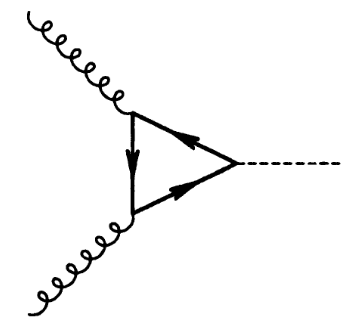
\includegraphics[scale=0.3]{ChapterTheory/figs/ggH.png}}
	\subfloat[]{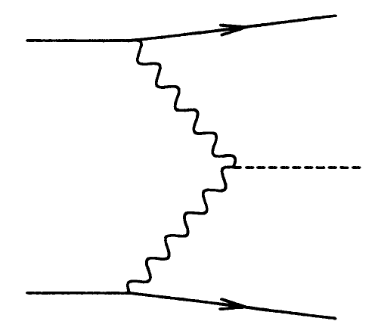
\includegraphics[scale=0.3]{ChapterTheory/figs/VBF.png}}
	\subfloat[]{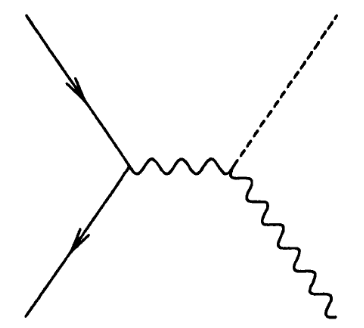
\includegraphics[scale=0.3]{ChapterTheory/figs/AssWZ.png}}
	\subfloat[]{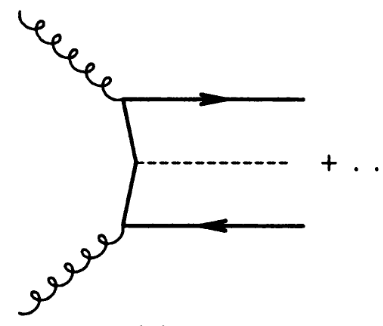
\includegraphics[scale=0.3]{ChapterTheory/figs/Ass_tt.png}}
	\legend{(a) gluon fusion; (b) vector boson fusion; (c) Higgs-strahlung; (d) associated production with top quark.}
	\source{ELLIS, 2003, p. 398.}
	\label{fig:Higgs_pro_mechanisms}
\end{figure}

The Feynman diagrams at LO (\textit{leading-order}) for each of this processes are shown in Fig.~\ref{fig:Higgs_pro_mechanisms}. The gluon fusion is the production mode in which the Higgs is produced through a loop of top quarks induced by the interaction of gluons in the initial state. This is the production mode with the highest probability to happen, presenting a cross section of about 43.9 pb for $m_{H} = $ 125GeV at $\sqrt{s} = $13TeV \cite{bib:LHC-Higgs-XSWG-2018}. 

The second most important production mode is the vector boson fusion. In this production mode the Higgs is created by the fusion of weak vectorial bosons ($Z$, $W^{\pm}$) which arises during the scattering of quarks in the colliding protons. The main characteristic of this mode is the presence of two energetic jets in the final state and separated by a pseudorapidity gap. Its cross section at 13TeV for $m_{H} = $125GeV is about 3.7 pb \cite{bib:LHC-Higgs-XSWG-2018,bib:IFAE-14-2008,bib:PhysRevD98-030001-2018}.

The cross section of the Higgs production associated to vectorial bosons is even smaller, but they are useful for observing the Higgs decaying into $b\bar{b}$ or $\gamma\gamma$ since the decay can be tagged by the presence of the bosons $W/Z$. The production of Higgs up to $M_{H} \sim 400~GeV$ associated to quark top is the smallest one between the main production modes. This process is similar to the Higgstrahlung, but the Higgs in this case is emitted from top quarks through $gg$ or $q\bar{q}$ interactions \cite{bib:ellis-2003}.

The Higgs can decay in several final states and each of them presents advantages and disadvantages. The decaying channel $ZZ \rightarrow 4l$, handled in this analysis, is one of the best ones. This channels is actually called "the golden channel" because all the decay products can be fully reconstructed in the CMS detector and it also has relatively small backgrounds at the signal region. However, the branching ratio (BR) into $ZZ \rightarrow 4l$ is small, about 3.3x10$^{-6}$ for $m_{H} = $125GeV at 13TeV \cite{bib:LHC-Higgs-XSWG-2018}. The Fig.~\ref{fig:Higgs_XSBR} shows in (a) the Higgs cross sections for different center-of-mass energies and in (b) its branching ratios at 13TeV (the energy in which this analysis have been done).

\begin{figure}[htbp]{15cm}
	\caption{Higgs production cross section and branching ratios.}
	\subfloat[]{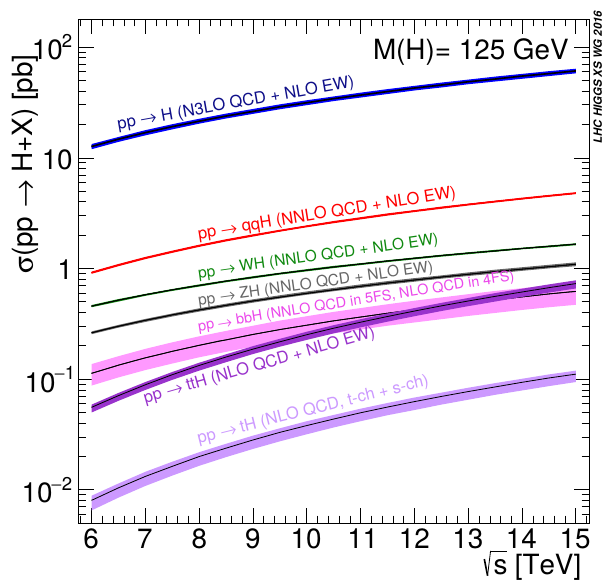
\includegraphics[scale=0.4]{ChapterTheory/figs/Higgs_XS_vs_S.png}}
	\quad
	\subfloat[]{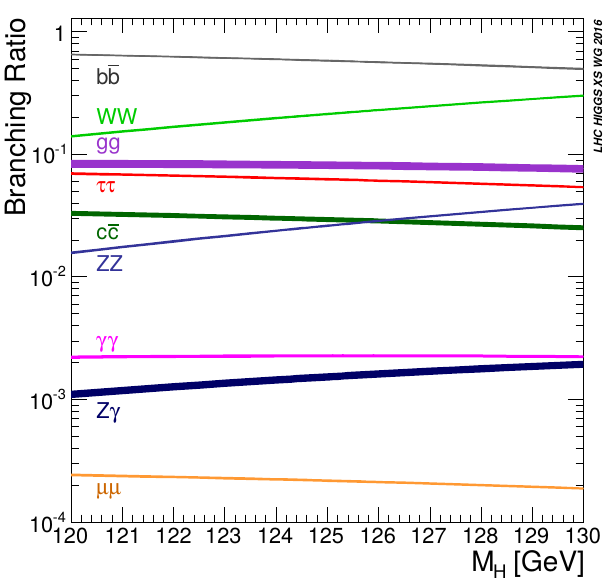
\includegraphics[scale=0.4]{ChapterTheory/figs/Higgs_BRs.png}}
	\legend{(a) cross sections as function of the center-of-mass energy; (b) branching ratios at $\sqrt{s}$ = 13 TeV.}
	\source{TANABASHI, 2018, p. 184.}
	\label{fig:Higgs_XSBR}
\end{figure}

\section{The Higgs VBF Production Mode \label{sec:vbf_theory}}
Many measurements of the properties of the Higgs boson are still statistics limited, and there is still significant room for beyond standard model effects in the Higgs sector. A particularly sensitive channel for observing non-standard model effects is the cross section for Higgs boson production through the Vector Boson Fusion (VBF) mode. There are some special features about this production mode. It has the largest cross section between the processes that involves tree-level production of the Higgs boson. It is also the second largest among all the processes. Its signature of two energetic forwarded jets makes possible to tag events and identify Higgs decays that normally have large backgrounds. Another feature is that the Higgs $p_{T}$ is nonzero, even at lowest order, facilitating searches of invisible decay modes. The VBF mode also has a particular sensitivity to the charge-parity properties of the Higgs boson and non-standard Higgs interactions via  the angular correlations between the jets \cite{bib:Dittmaier_et_al_2011,bib:Dittmaier_et_al_2012,bib:Dittmaier_et_al_2013,bib:CMS-PAS-HIG-14-038,bib:ATLAS-CONF-2015-004,bib:PhysRev88-051801-2002}.

\subsection{The Higgs VBF LO Cross Section and its Kinematics}
\begin{figure}[htbp]{15cm}
	\caption{Feynman diagram for the Higgs production via vector boson fusion. The initial state quarks (or anti-quarks) are $p_{1}$ and $p_{2}$, while the momentum at final state are $p_{1}'$ and $p_{2}'$, respectively.}
	\begin{overpic}
		[scale=0.35]{ChapterTheory/figs/VBF}
		\put(-5,80){$p_{1}$}
		\put(-5,10){$p_{2}$}
		\put(100,85){$p_{1}'$}
		\put(100,5){$p_{2}'$}
		\put(100,45){$H$}
		\put(60,55){$V$}
		\put(60,20){$V$}
	\end{overpic}
	\source{CAHN, 1984, p. 196. Adapted by the author.}
	\label{fig:vbf_labeled_diagram}
\end{figure}

Assuming the Higgs production via the VBF mode as shown in Fig.~\ref{fig:vbf_labeled_diagram}, the matrix element for this process, in terms of the momentum of the involved particles, can be expressed as \cite{bib:PhysLettB136-3-1984}

\begin{equation}
\mathcal{M} = g_{VVH}~\frac{\bar{u}(p_{1}')\gamma^{\lambda}(g_{V}+g_{A}\gamma_{5})\bar{u}(p_{1})~\bar{u}(p_{2}')\gamma_{\lambda}(g_{V}'+g_{A}'\gamma_{5})\bar{u}(p_{2})}{(q_{1}^{2}-M_{V}^{2})~(q_{2}^{2}-M_{V}^{2})},
\end{equation}

where for,

\begin{multicols}{2}
$V = W$:
\begin{eqnarray}
g_{VVH} \rightarrow g_{WWH} = gM_{W}\\
g_{V} = -g_{A} = \frac{e}{2\sqrt{2}~sin~\theta_{W}}
\end{eqnarray}
$V = Z$:
\begin{eqnarray}
g_{VVH} \rightarrow g_{ZZH} = \frac{gM_{W}}{cos^{2}\theta_{W}}\\
g_{V} = \frac{g(T_{3L}/2 - Q~sin^{2}\theta_{W})}{cos~\theta_{W}}\\
g_{A} = - \frac{gT_{3L}}{2~cos~\theta_{W}}.
\end{eqnarray}
\end{multicols}

The term $g = e/sin~\theta_{W}$ is the weak SU(2) gauge coupling and the terms $T_{3L}$ and $Q$ stand for the third component of the weak isospin and the quark charge\footnote{For quarks and leptons $T_{3L} \pm 1/2$.}, respectively. Now, using $g_{L} = (g_{V}-g_{A})/2$ and $g_{L} = (g_{V}+g_{A})/2$ the average squared matrix element becomes \cite{bib:PhysLettB136-3-1984,bib:PhysRep457-1-2005,bib:NuclPhysB287-1987}

\begin{equation}
|\mathcal{M}|^{2} = 64~g_{VVH}^{2}~\frac{C_{1}(p_{1}.p_{2})(p_{1}'.p_{2}') + C_{2}(p_{1}.p_{2}')(p_{1}'.p_{2})}{(q_{1}^{2}-M_{V}^{2})^{2}~(q_{2}^{2}-M_{V}^{2})^{2}}
\end{equation}

where $C_{1} = g_{L}^{2}g_{L}^{'2} + g_{R}^{2}g_{R}^{'2}$ and $C_{1} = g_{L}^{2}g_{R}^{'2} + g_{R}^{2}g_{L}^{'2}$. The differential cross section at LO is, then, given by \cite{bib:PhysRep457-1-2005}

\begin{equation}
d\hat{\sigma}_{LO} = \frac{1}{72}\frac{1}{(2\pi)^{5}}\frac{1}{\hat{s}}~|\mathcal{M}|^{2}~\frac{d^{3}p_{H}}{2dE_{H}}~\frac{d^{3}p_{1}'}{2dE_{1}'}~\frac{d^{3}p_{2}'}{2dE_{2}'}~\delta^{4}(p_{1}+p_{2}-p_{1}'-p_{2}'-p_{H})
\end{equation}

in which the integration over the variables $p_{1}'$ and $p_{2}'$ is conveniently performed in the rest frame of the final-state quarks ($\vec{p}_{1}' + \vec{p}_{2}' = 0$), leading to \cite{bib:PhysRep457-1-2005}

\begin{equation}
\frac{d\hat{\sigma}_{LO}}{dE_{H}~dcos~\theta} = \frac{G_{F}^{3}M_{V}^{8}}{9\sqrt{2}\pi^{3}\hat{s}}~\frac{p_{H}}{32s_{1}s_{2}}~(C_{1}\mathcal{H}_{1} + C_{2}\mathcal{H}_{2})
\label{eq:vbf_dxs_lo}
\end{equation}

where $\hat{s} = (p_{1}+p_{2})^{2}$ is the energy at the CM (\textit{center of mass}), $G_{F}$ is the Fermi constant, $s_{1,2} = \sqrt{\hat{s}}[(\sqrt{\hat{s}}-E_{H}) \pm p_{H}cos~\theta]$, with $p_{H}$ being the Higgs momentum and $\theta$ the final-state parton scattering angle\footnote{Do not confuse that with the $\theta_{W}$, which is the weak-mixing angle (Weinberg angle).}. The $\mathcal{H}_{1,2}$ are terms depending on $s_{1,2}$, $\hat{s}$, $p_{H}$, $\theta$ and $M_{V}$. For the interested reader, please see \cite{bib:PhysRep457-1-2005}.

The total partonic cross section of the Higgs produced via VBF is obtained by integrating the Eq.~\ref{eq:vbf_dxs_lo}, which can properly be done in terms of the Higgs transverse momentum and rapidity as

\begin{equation}
\hat{\sigma}_{LO}(qq \rightarrow Hqq) = \int_{y-}^{y+}dy~\int_{0}^{p_{T}^{max}}dp_{T}~(2\pi p_{T})~\frac{d^{2}\hat{\sigma}_{LO}}{dydp_{T}}.
\label{eq:vbf_xs_lo}
\end{equation}

The integration on $y$ and $p_{T}$ on Eq.~\ref{eq:vbf_xs_lo} can not be done analytically and numerical integration is used to get physical results \cite{bib:PhysRep457-1-2005,bib:NuclPhysB287-1987}. As reported on this previous references, the results show that the quarks at the final state present large energies while their transverse momentum is usually $p_{T} \sim M_{V}$ but, varying with $m_{H}$ (see Fig.~3.14 of \cite{bib:PhysRep457-1-2005} and Fig.~6 of \cite{bib:NuclPhysB287-1987}, for instance). The relatively small transverse momentum of the final-state partons can be translated into a small scattering angles, which in terms of pseudorapidity ($\eta$), means that, the rising jets are forward (a well known signature of VBF).


\subsubsection{Corrections of Higher Orders}
Through the past years considerable enhancements have been achieved in the phenomenological interpretation of the Higgs VBF production mode. Computations for the total cross section and differential distributions to Higgs produced via VBF and including NLO QCD and EW corrections were presented by \cite{bib:Phys46-203-1998,bib:PhysRevLett69-3274-1992} and are available in flexible parton-level Monte Carlo (MC) generators. Partial NNLO QCD corrections have also been presented by \cite{bib:PhysRevD77-053010-2008,bib:PhysRevLett105-011801-2010}, which reduces the uncertainties on the inclusive VBF cross section from 5-10$\%$ to 1-2$\%$, making VBF the theoretically most accurate production mode at hadron colliders \cite{bib:ChinPhysC-38-9-2014}. 

The most recent developments done on the VBF theory formalism comes from the application of the so called \textit{structure function approach}, which is based on the description, in very good approximation, of the VBF process as a double deep-inelastic scattering process (DIS), see Fig.~\ref{fig:vbf_DIS_approx}. In such approximation the two virtual vector bosons $V*_{1,2}$ are independently emitted from the hadronic initial states and fuse into the Higgs boson. 

\begin{figure}[htbp]{15cm}
	\caption{Sketch of the Higgs VBF production description through the structure function approach.}
	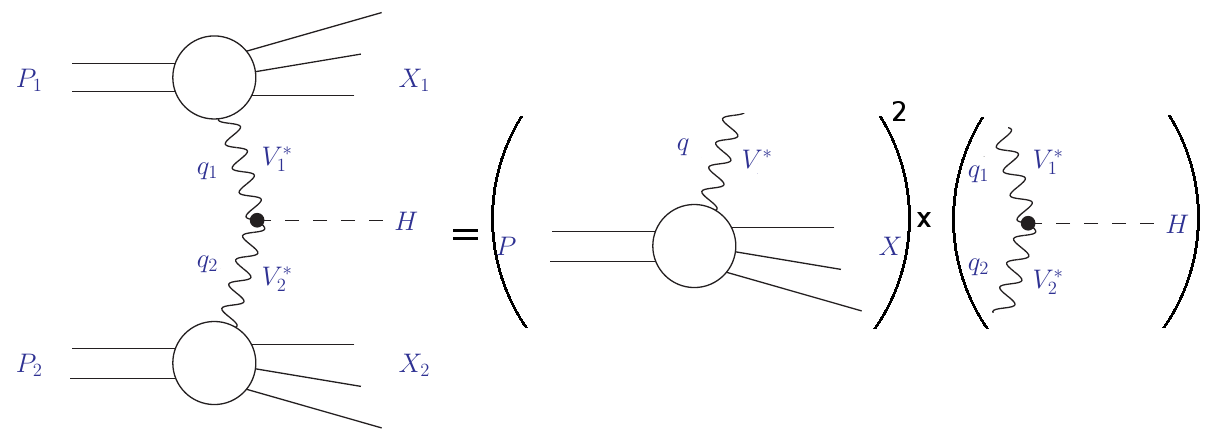
\includegraphics[scale=0.4]{ChapterTheory/figs/vbf_DIS_approximation}
	\source{BOLZONI, 2010, p. 3. Adapted by the author.}
	\label{fig:vbf_DIS_approx}
\end{figure}

This approximation builds on the absence (or smallness) of QCD interference between the two inclusive final states $X_{1}$ and $X_{2}$. The total cross section is given as a product of the matrix element $\mathcal{M}^{\mu\nu}$ for VBF ($V_{1}^{\mu}V_{2}^{\nu} \rightarrow H$) and the DIS hadronic tensor $W_{\mu\nu}$, giving a VBF differential cross section of the form \cite{bib:PhysRevLett105-011801-2010,bib:PhysRevLett69-3274-1992},

\begin{eqnarray}
\nonumber
d\sigma = \frac{1}{2s}2G_{F}^{2}~M_{V_{1}}^{2}M_{V_{2}}^{2}~\frac{1}{(Q_{1}^{2}+~M_{V_{1}}^{2})^{2}}~\frac{1}{(Q_{2}^{2}+~M_{V_{2}}^{2})^{2}}\times\\
\nonumber
W_{\mu\nu}(x_{1},Q_{1}^{2})\mathcal{M}^{\mu\rho}\mathcal{M}^{*\nu\sigma}W_{\rho\sigma}(x_{2},Q_{2}^{2})\times\\ \frac{d^{3}P_{X_{1}}}{(2\pi)^{3}2E_{X_{1}}}~\frac{d^{3}P_{X_{2}}}{(2\pi)^{3}2E_{X_{2}}}~ds_{1}ds_{2}~\frac{d^{3}P_{H}}{(2\pi)^{3}2E_{H}}
(2\pi)^{4}~\delta^{4}(P_{1}+P_{2}-P_{X_{1}}-P_{X_{2}}-P_{H}),
\label{eq:vbf_dis_differential_XS}
\end{eqnarray}

where, $s$ stands for the center-of-mass energy of the collider, $G_{F}$ is the Fermi's constant, $Q_{1}^{2} = -q_{i}^{2}$ and $x_{i} = Q_{i}^{2}/(2P_{i}.q_{i})$ are the usual DIS variables, $M_{V_{i}}$ stands for the vector boson mass. The hadronic tensor $W_{\mu,\nu}$ represents the unknown physics at the $V_{\mu,\nu}^{1,2}$-parton vertexes. This function depends on the four-momentum of both vector boson and the parton. 

The theoretical discussion about the full computation of the total cross section exceeds the scope of this analysis and it will not be presented here. For the reader interested in more details, please have a look on \cite{bib:PhysRep457-1-2005}, \cite{bib:PhysRevLett69-3274-1992} and \cite{bib:PhysRevLett105-011801-2010}.


\section{The Physics Scenario of this Analysis}
The VBF production mode, as presented on previous sections, is a key process for precision measurements of Higgs properties since it is a clean channel with very distinctive kinematics. Such features provide good scenario for measurements of Higgs couplings \cite{bib:PhysRevD62_013009_2000}. The VBF channel is a direct probe of the coupling between vector bosons and the Higgs boson, and hence directly probes the electroweak sector of the standard model.

Additionally, the $H \rightarrow ZZ \rightarrow 4l$ (l = e, $\mu$) decay channel has a large signal-to-background ratio because it is possible to completely reconstruct the final state leptons, which presents excellent momentum resolution. This feature makes this decay channel one of the most important for the studies of the Higgs boson properties. Several different measurements have been performed with the data collected during the LHC RunI using this channel
\cite{bib:PhysRevLett110-081803-2013,bib:PhysRevD89-092007-2014,bib:PhysLettB-736-64-2014,bib:PhysRevD92-012004-2015,bib:PhysRevD92-072010-2015}. This decay channel, thus, presents a good frame to measure Higgs VBF production.

This analysis presents a measurement of the Higgs boson VBF production cross-section obtained in the $H \rightarrow ZZ \rightarrow 4l$ decay channel using data collected at $\sqrt{s}=$ 13TeV. The data accounts for 35.9$fb^{-1}$ of pp collision collected with the CMS detector at the LHC RunII in 2016. This analysis uses similar requirements as the CMS $HZZ4L$ 2016 analysis \cite{bib:CMS-AN-16-442} and \cite{bib:CMS-AN-16-328}, relying essentially on the reconstruction, identification and isolation of leptons and requiring the presence of jets and Missing Energy Transverse (MET). The specific selection and analysis requirements will be discussed in more detail in the following sections.

As it will also be shown, the main processes in this analysis, besides the VBF itself, are the $gg \rightarrow H$ Higgs production mode and the reducible SM background $q\bar{q} \rightarrow ZZ$ (which in the context of the present analysis become a non-reducible background). In a smaller, but still significant, contribution appears the remaining Higgs production modes, Higgs-strahlung (VH) and associated with top quark ($t\bar{t}H$), and the SM background $gg \rightarrow ZZ$. The tree-level Feynman diagrams for each of these processes are shown in Fig.~\ref{fig:processes_feynman}.

\begin{figure}[htbp]{16cm}
	\caption{Main physic processes in this analysis.}
	\centering
	\subfloat[]{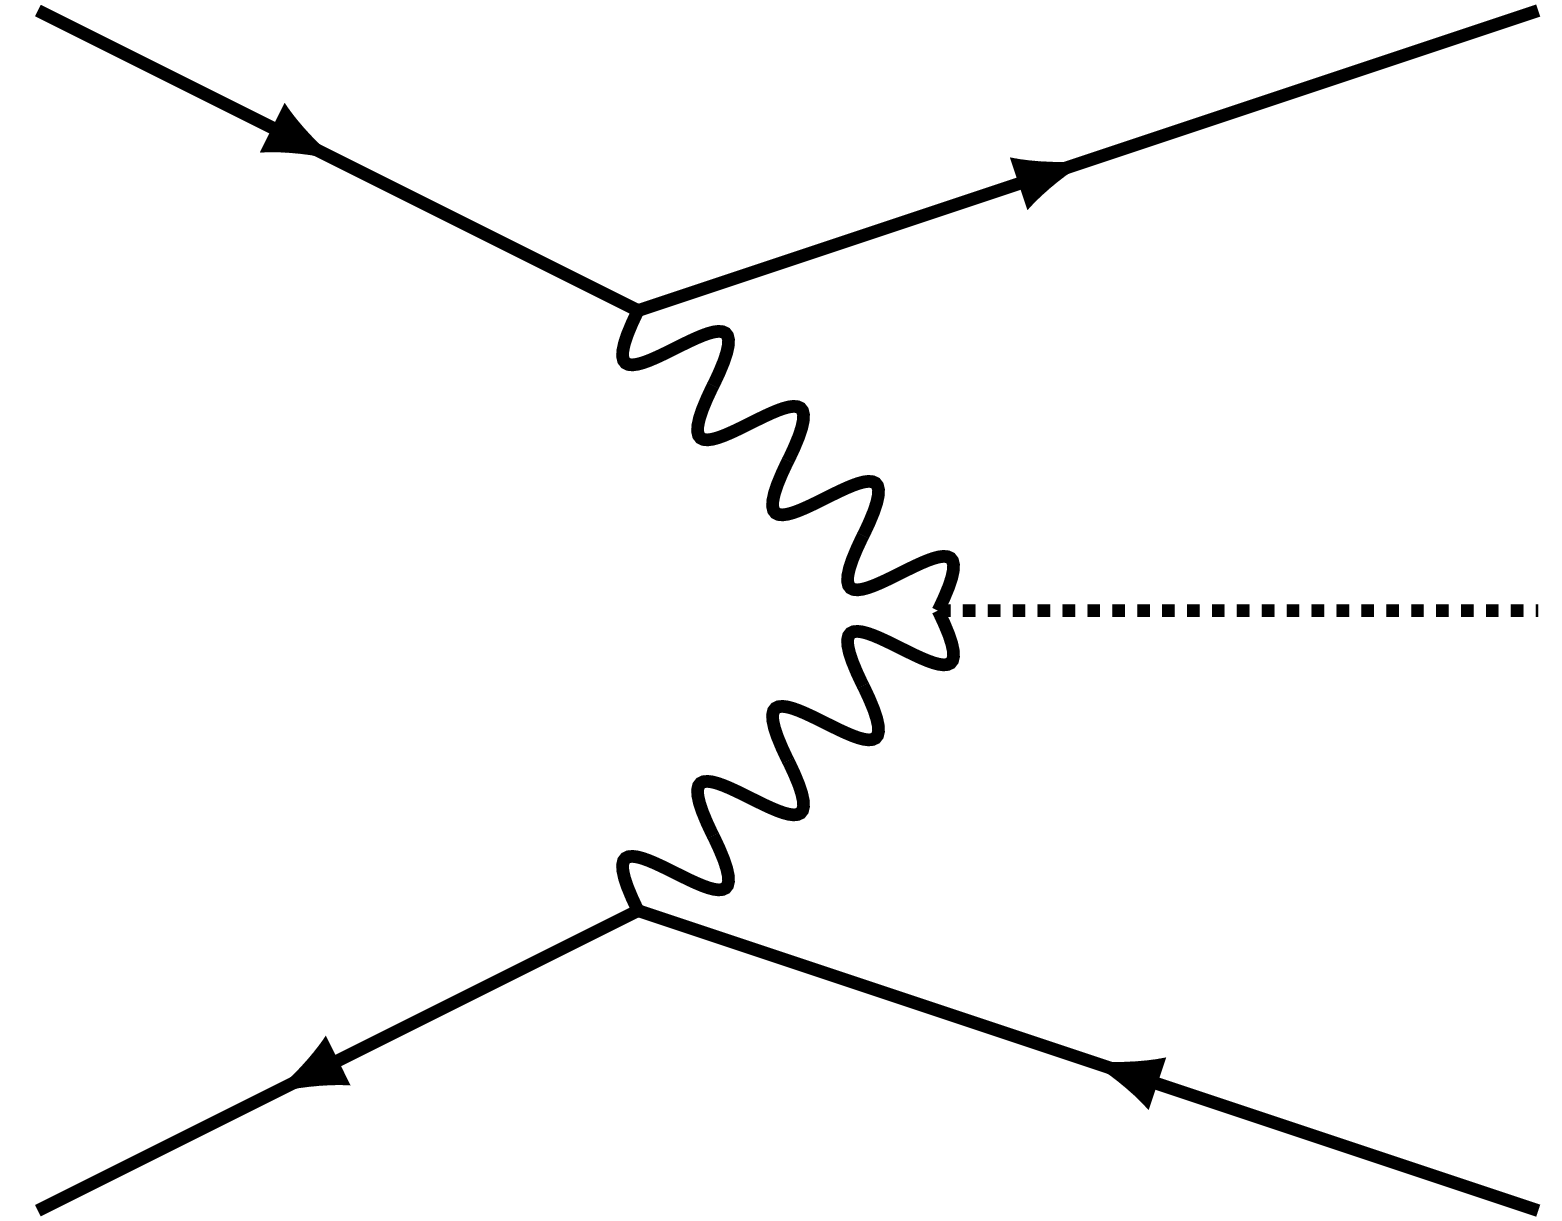
\includegraphics[scale=0.08]{ChapterAnalysis/figs/vbf_diagram}}
	\quad\quad
	\subfloat[]{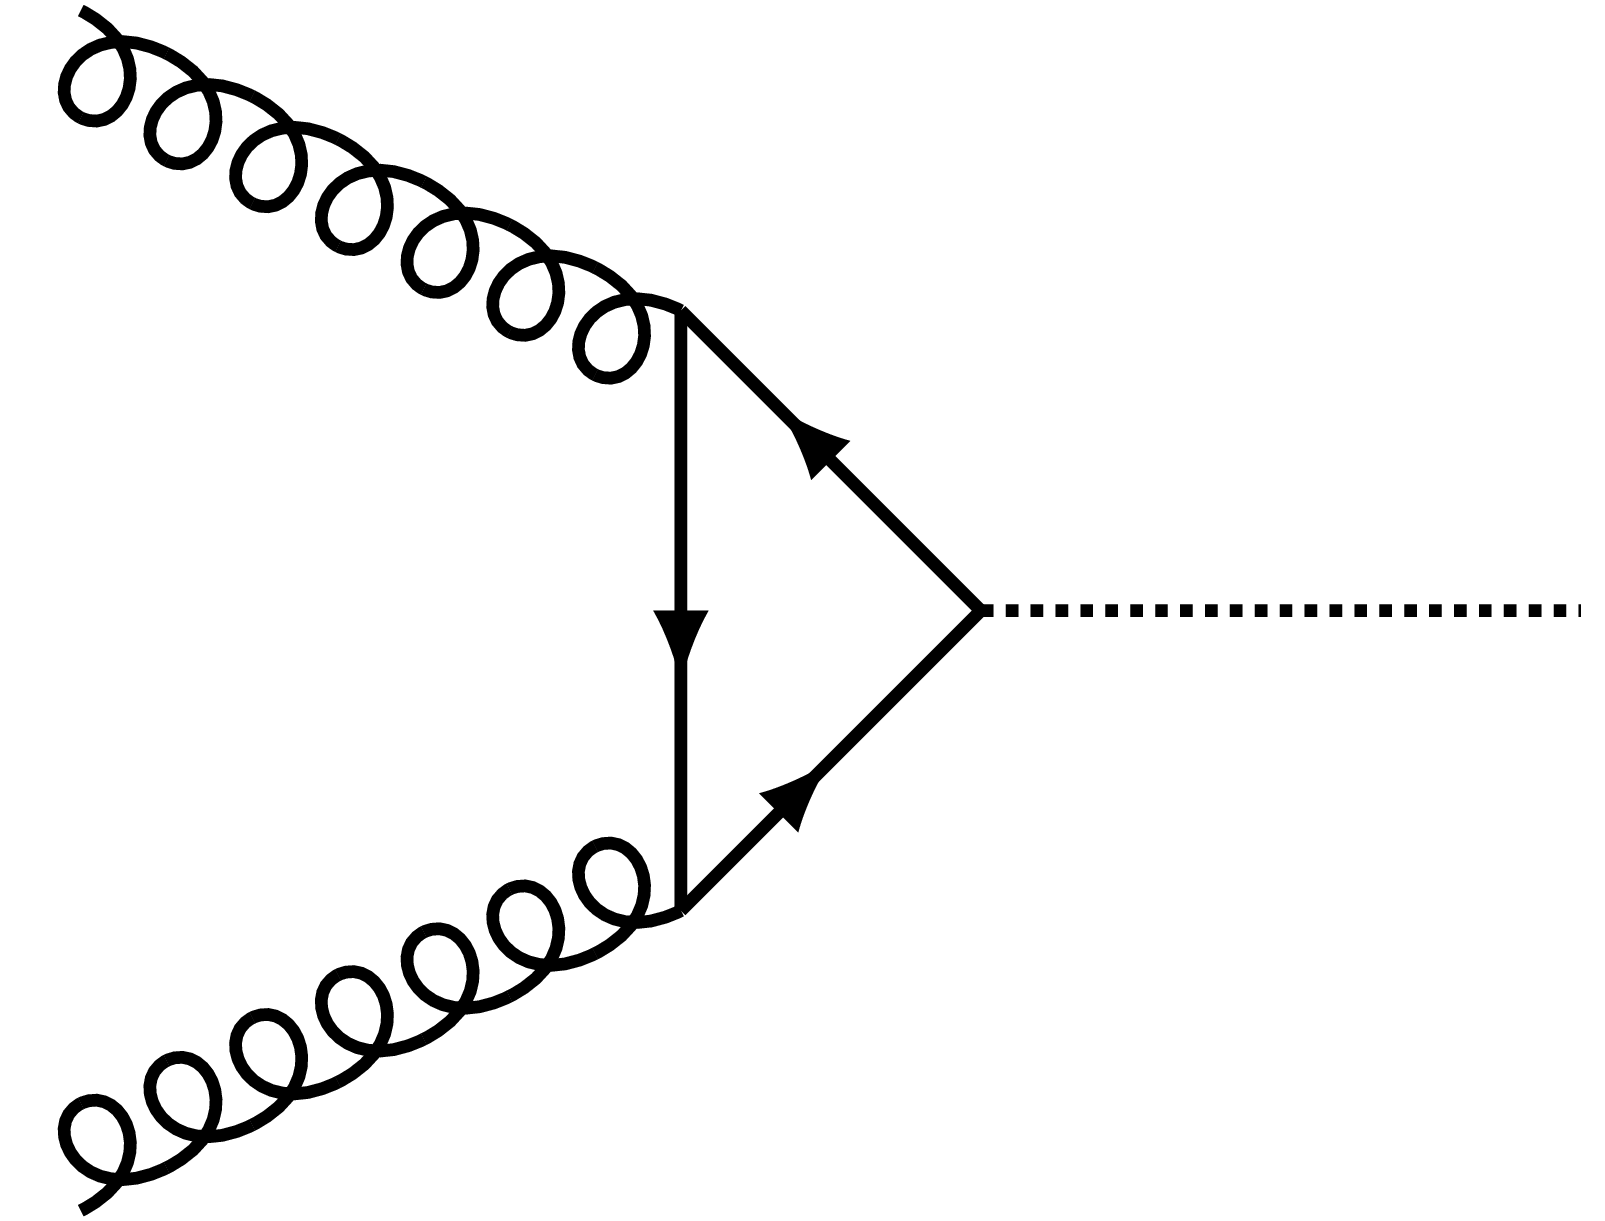
\includegraphics[scale=0.08]{ChapterAnalysis/figs/ggh_diagram}}
	\quad\quad
	\subfloat[]{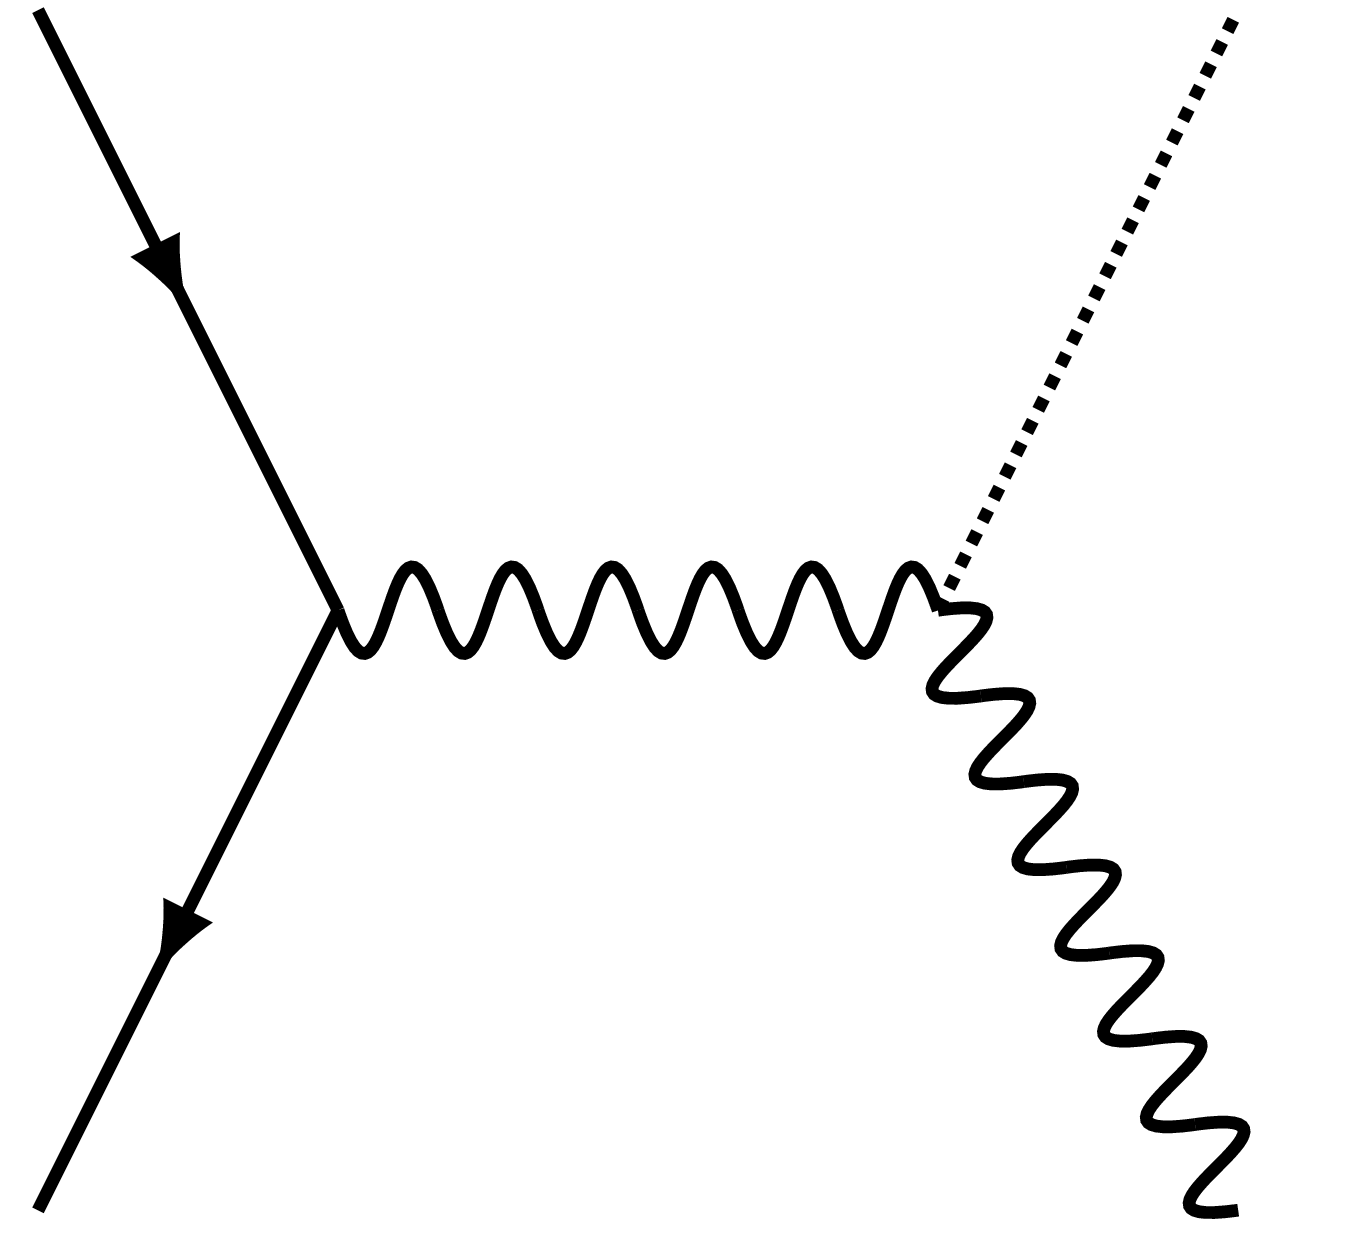
\includegraphics[scale=0.08]{ChapterAnalysis/figs/vh_diagram}}\\
	\subfloat[]{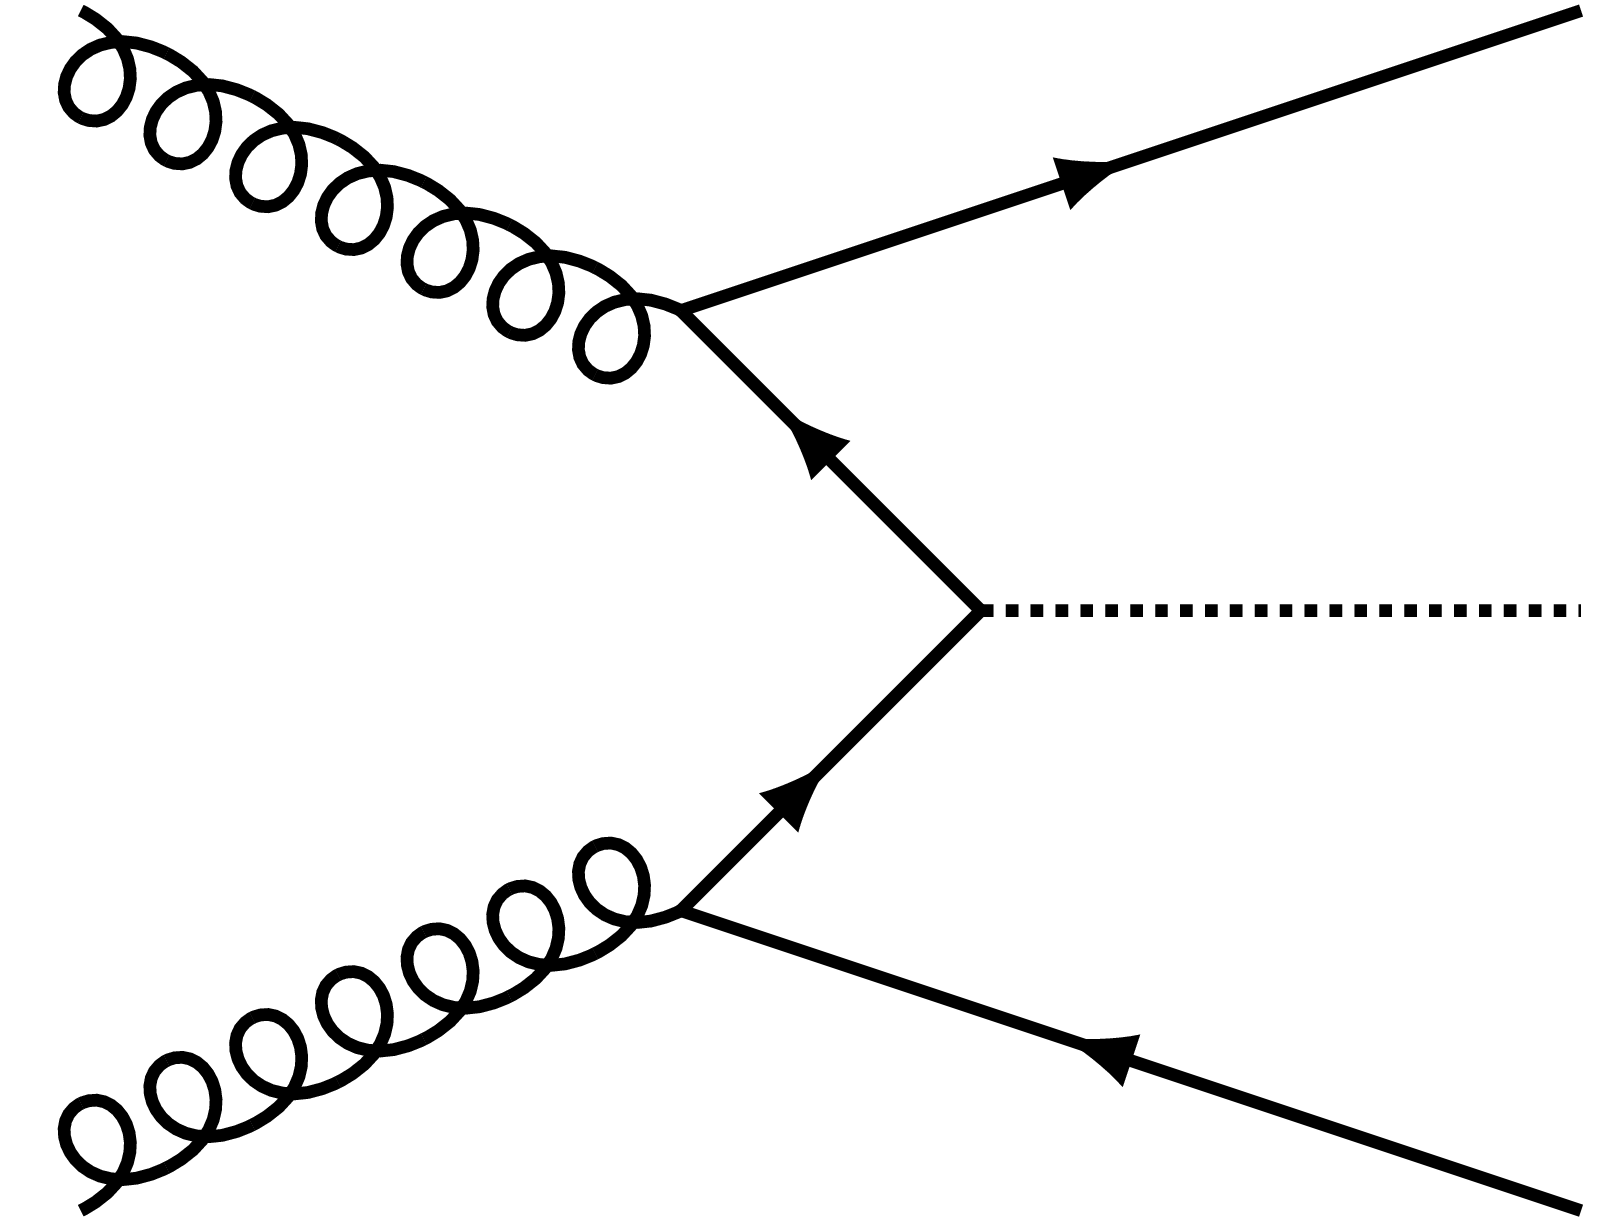
\includegraphics[scale=0.08]{ChapterAnalysis/figs/tth_diagram}}
	\quad\quad
	\subfloat[]{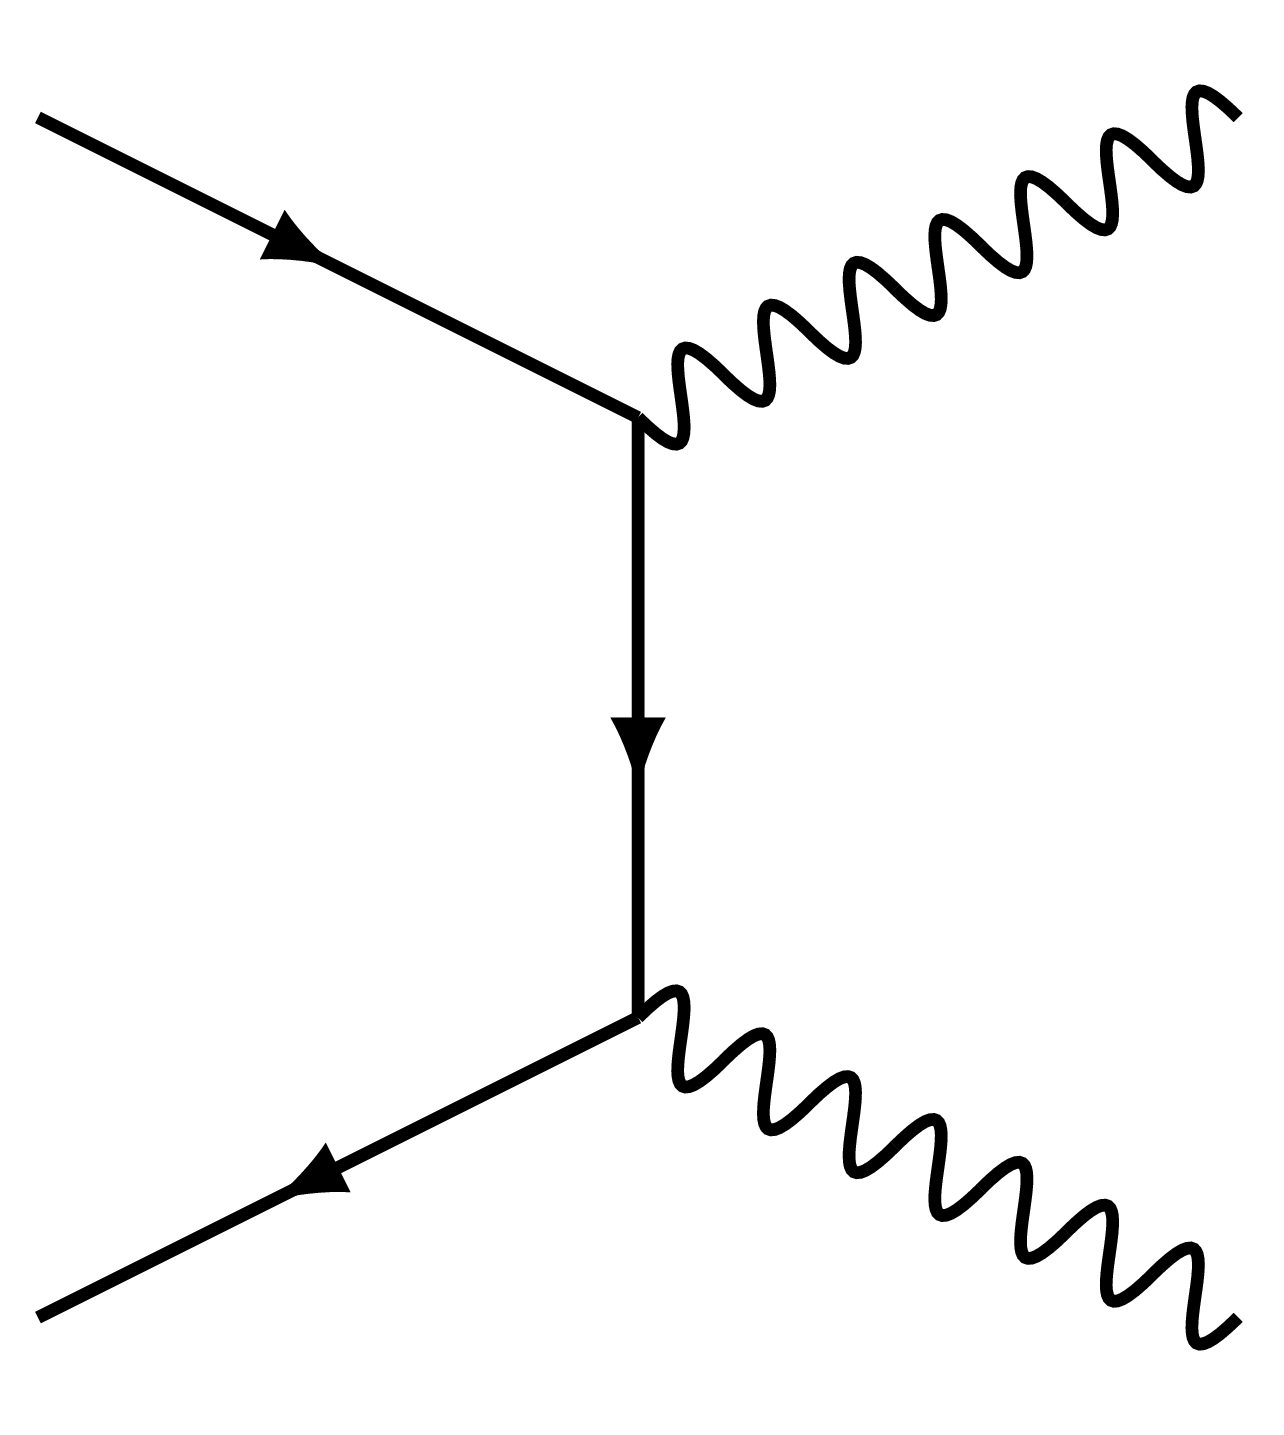
\includegraphics[scale=0.08]{ChapterAnalysis/figs/qqzz_diagram}}
	\quad\quad
	\subfloat[]{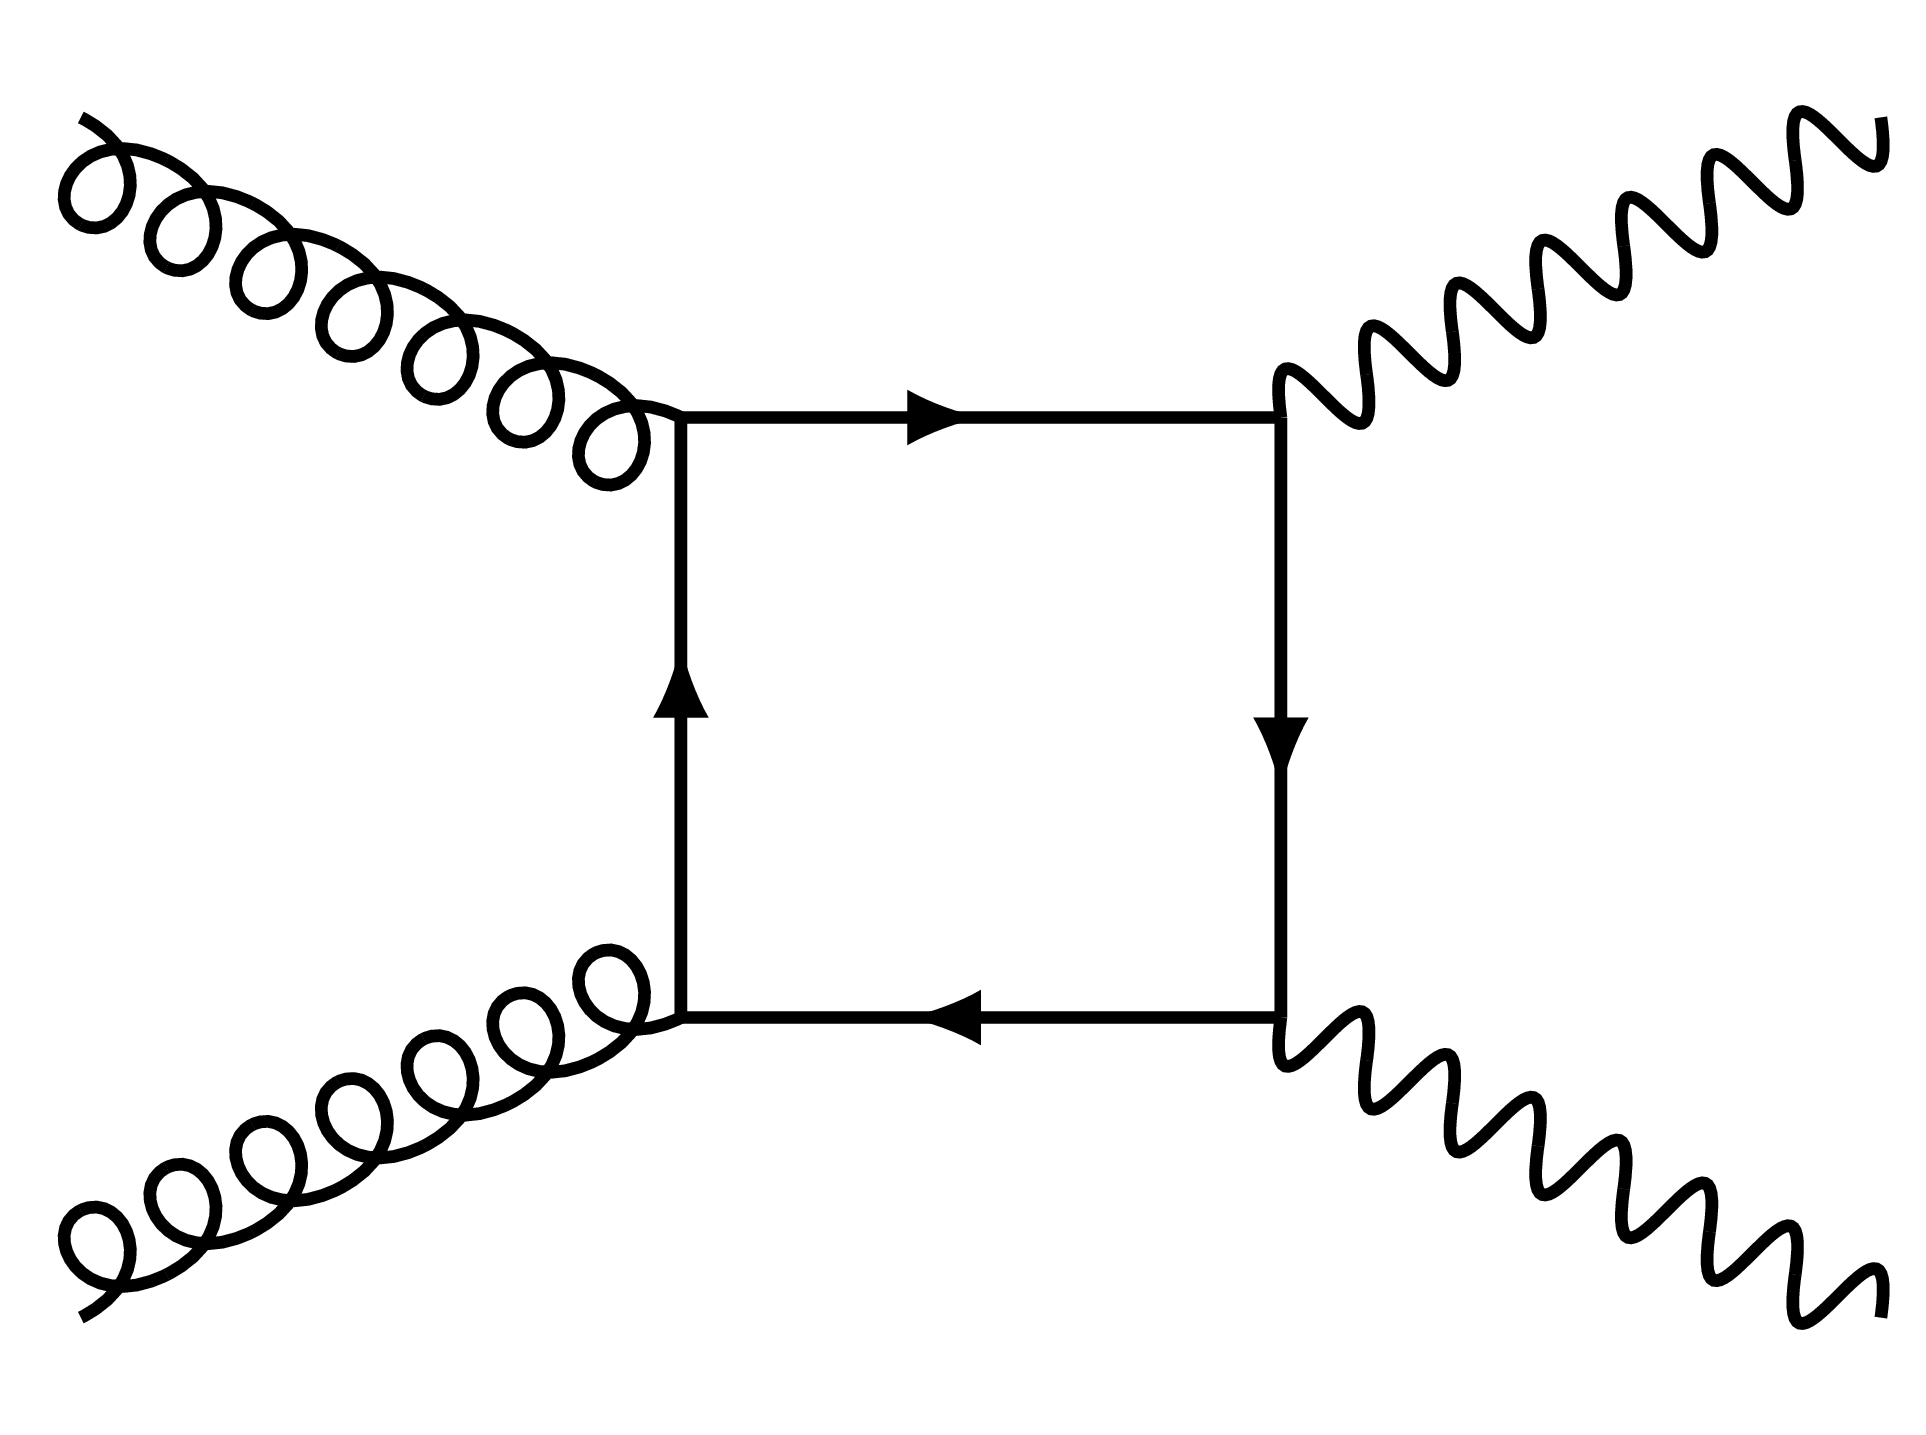
\includegraphics[scale=0.08]{ChapterAnalysis/figs/ggzz_diagram}}
	\label{fig:processes_feynman}
	\legend{(a) $q\bar{q} \rightarrow Hq\bar{q}$: vector boson fusion (VBF); (b) $gg \rightarrow H$: gluon-fusion (ggH); (c) $q\bar{q} \rightarrow VH$: Higgsstrahlung (VH); (d) $gg \rightarrow t\bar{t}H$: production associated to top quark; ZZ backgrounds (e) $q\bar{q} \rightarrow ZZ$ and (f) $gg \rightarrow ZZ$. Additionally there is the $Z+X$ background (not in the picture) which is derived via the Fake Rate \textit{data-driven} method and will be presented later.}
	\source{The author, 2018.}
\end{figure}
